% 负向 fixture：子节点超出所属 zone 容器（node-outside-zone）。
% 经典 mode-A 失败：真实内容比 skeleton 固定宽度长 → 子框溢出 zone。
% 刻意设计为「只触发 node-outside-zone 一类 error」以专门守护该检测：
%   - zone 只填充、不描边（无 border line → 不会顺带触发 line-through-node）
%   - 两个安分子框让该填充被识别为 zone（holds >=2 centers）
%   - 第三个子框过宽 → 左右各溢出 ~42pt
% 若 pdf-overlap-checker 不再报 node-outside-zone，说明该几何门被削弱。
% 纯英文 + plain tikz，任意机器可编译。
\documentclass[border=4pt]{standalone}
\usepackage{tikz}
\begin{document}
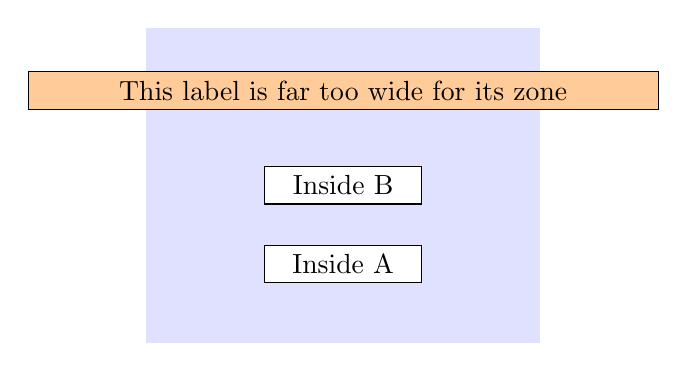
\begin{tikzpicture}
  \fill[blue!12] (0,0) rectangle (5,4);                       % zone (fill only)
  \node[draw, fill=white, minimum width=2cm] at (2.5,1) {Inside A};
  \node[draw, fill=white, minimum width=2cm] at (2.5,2) {Inside B};
  \node[draw, fill=orange!40, minimum width=8cm] at (2.5,3.2)
    {This label is far too wide for its zone};
\end{tikzpicture}
\end{document}
